% !TEX root = ../notes_template.tex
\chapter{Renal Clearance}\label{chp:blood_content}
Updated on \today
\minitoc

This chapter covers the concept of mass balance with a particular focus on water and electrolyte mass balance. The mass balance of water and electrolytes are supported by renal clearance which includes filtration, reabsorption and secretion for the formation and excretion of urine. Water and electrolyte mass balance are importance processes in the support of plasma (and therefore blood) volume and the concentration of electrolytes in the extra-cellular fluid. In Chapter \ref{chp:ecf_microcirculation} it was clear that alterations in the plasma volume and concentration become transferred to the interstitial fluid and from there to the ICF. The regulation of body fluid volume and composition is accomplished by acting directly on the plasma. The kidneys (and other systems such as the gastrointestinal, metabolic, and pulmonary) participate in the regulation of the body fluid volume and composition by acting on the plasma.

\vspace{5mm}

\textbf{Objectives include:}
\begin{enumerate}
    \item
    \item
    \item
    \item
    \item
\end{enumerate}

\section{Mass Balance}

This chapter is the first to specifically discuss the concept of mass balance. Mass balance applies the conservation of mass and energy to the analysis of physical systems. It considers the mass and energy entering (inputs) and leaving a system (outputs). For the physical therapist the need for inputs into the human system is one reason for human function. To use the terms from the ICF model introduced in the Introduction, the inputs of food, drink and air require activity and participation (function). Many activities of daily living (ADLs) are based on the functional activities that provide appropriate inputs, and hygienic outputs required for physiological mass balance.

The inputs of food, drink and air ultimately provide the water, nutrients (macronutrients and micronutrients) and oxygen that are utilized for physiological processes. An overview of physiological mass balance is provided in Figure \ref{fig:mass_balance}. How these are used, whether they can be recycled, and the ways in which they are lost influences the time scale of the need for inputs. When describing outputs the term incidental loss refers to loss that occurs without purpose. Incidental loss is contrasted with intentional loss. An example of incidental loss is the loss of Na++ in sweat. The loss of water with sweat is purposeful as part of thermoregulation. But the loss of Na++ with sweat is unnecessary for the primary purpose of thermoregulation, but still requires replacement of Na++. Loss due to use such as oxygen in ETC, or due to a role being played in excretion of waste products such as water in feces and urine, is intentional loss. 

\begin{figure}[!h]
    \centering
    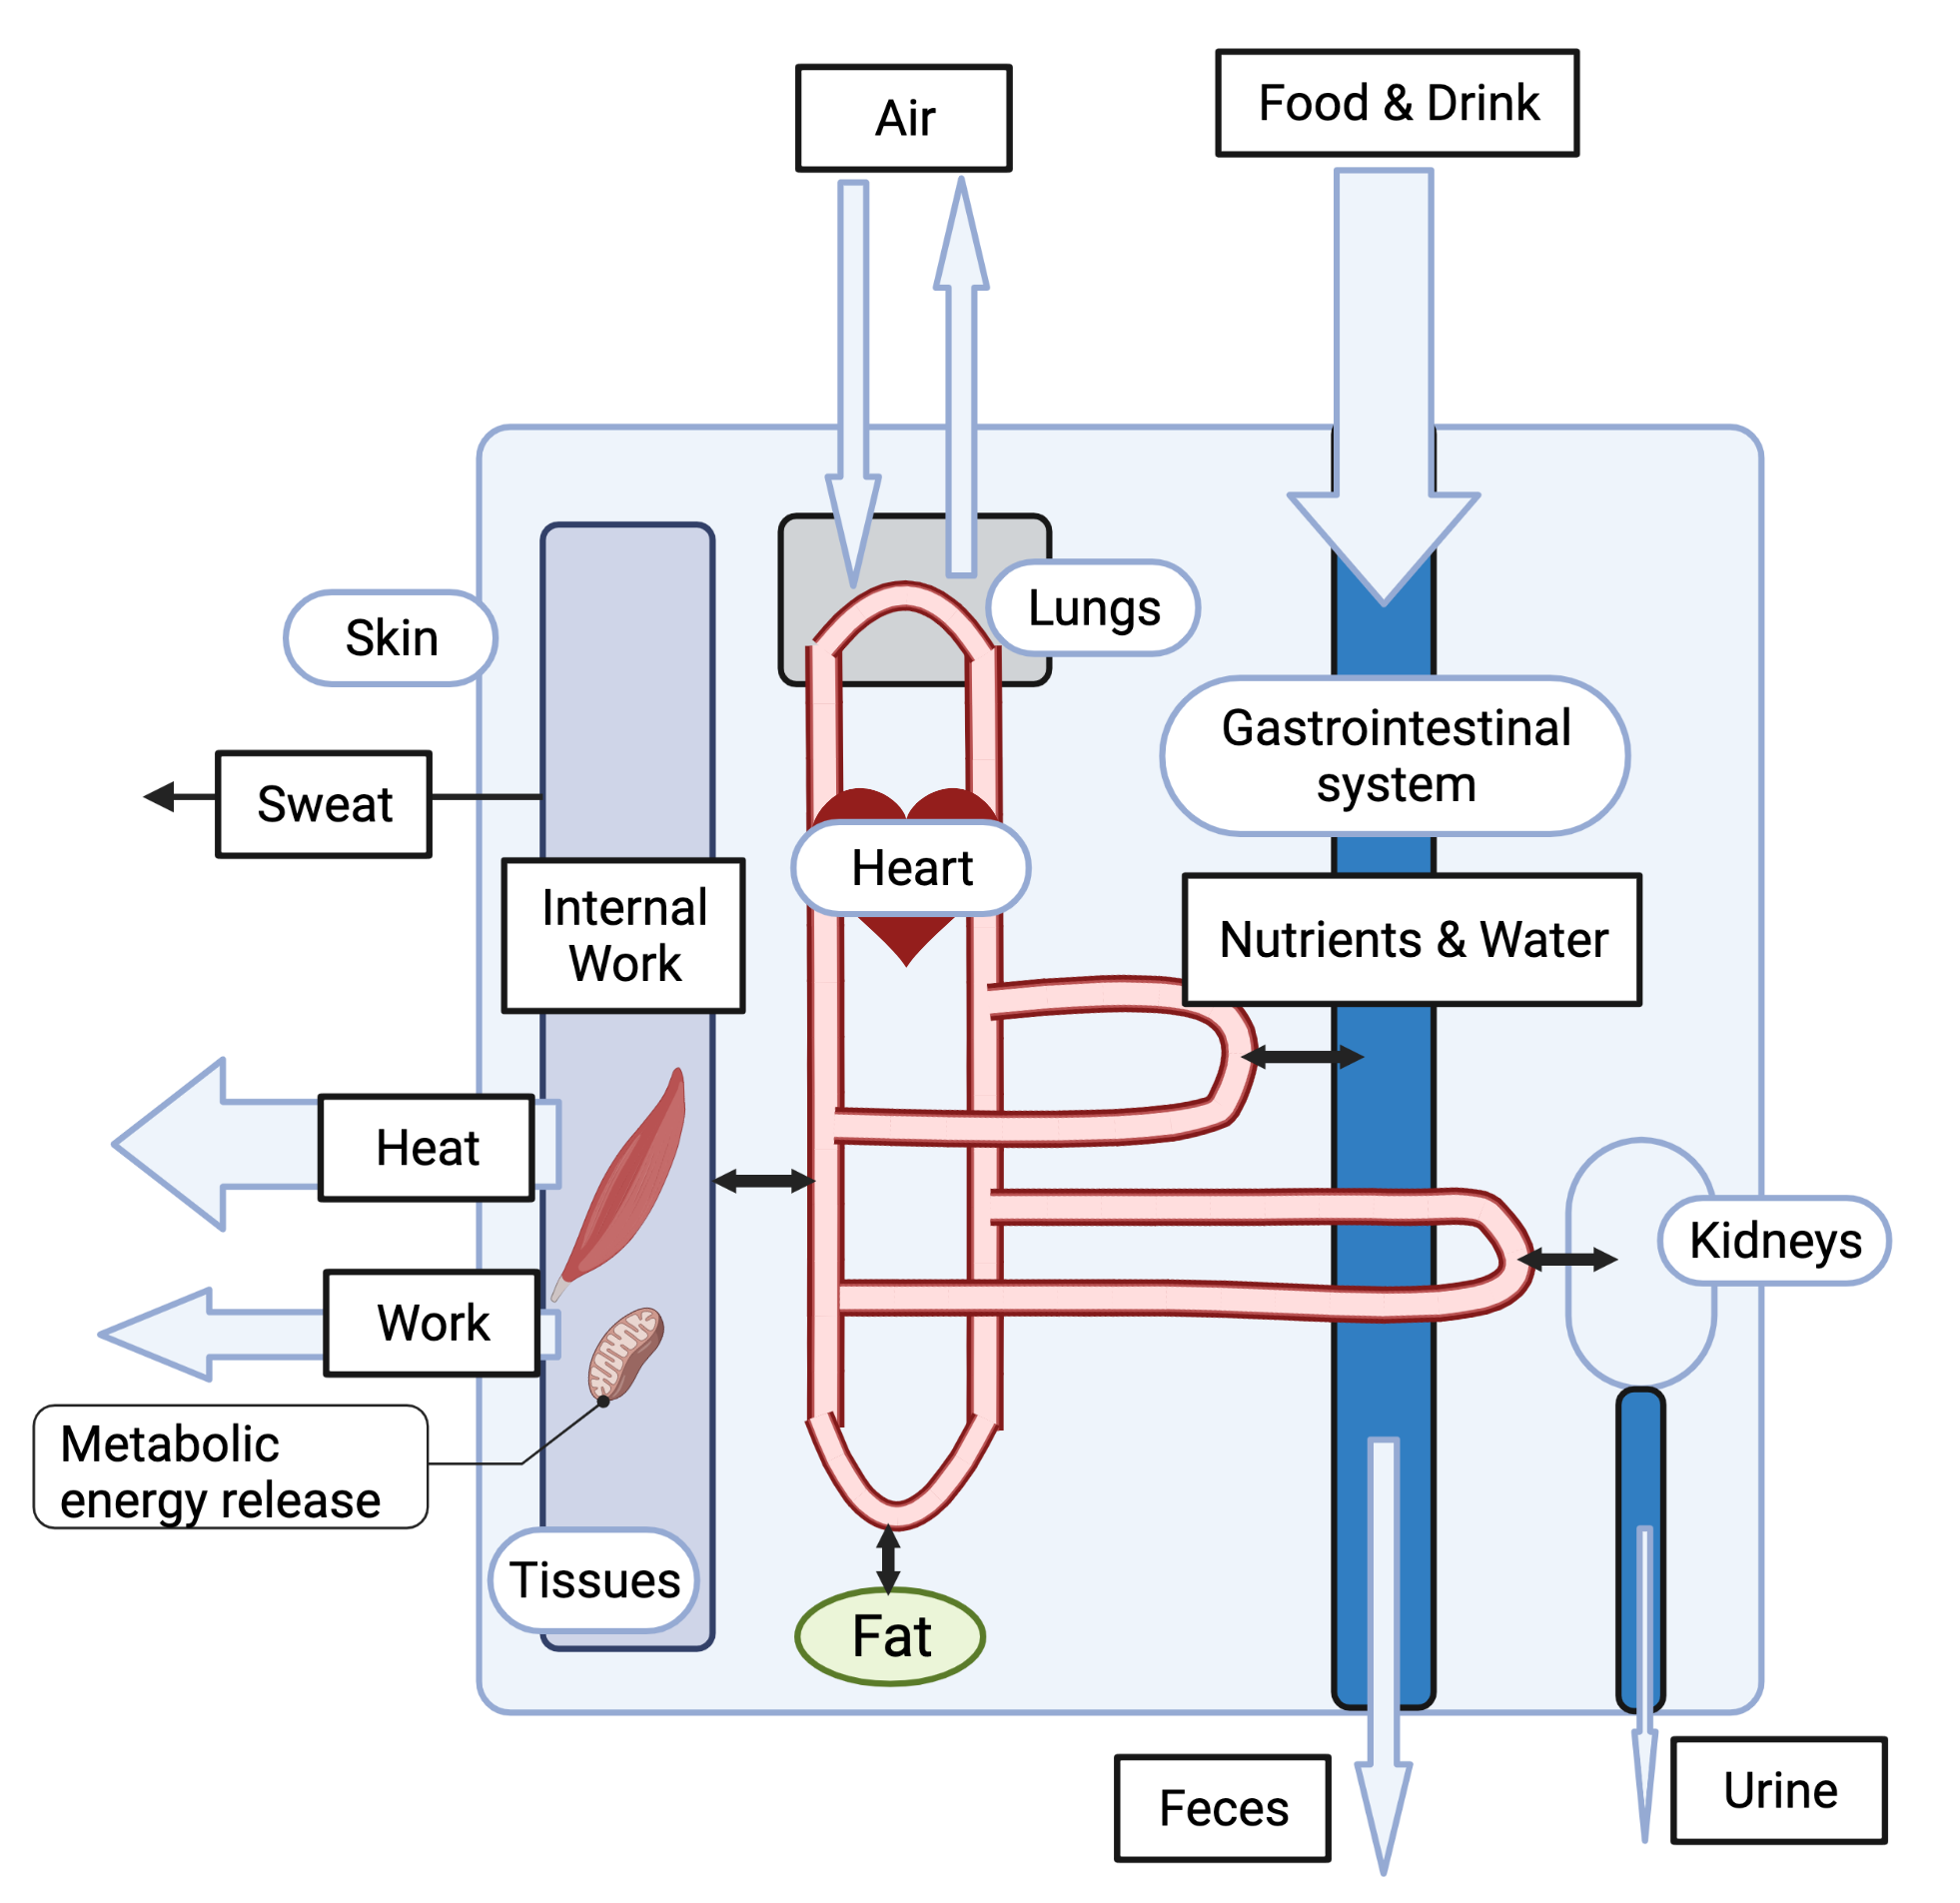
\includegraphics[width=1\linewidth]{./figure/mass_balance.png}
    \caption{Physiological Mass Balance \footnotesize{(Created with BioRender.com)}}
    \label{fig:mass_balance}
\end{figure}

\subsection{Oxygen Mass Balance}
Oxygen is used regularly and relatively quickly with very little storage (myoglobin) and no recycling, making the input of air with oxygen a regular requirement. Life is not sustainable for prolonged periods without the input of air over the time scale of a few minutes in most individuals. At nearly the same rate, and at times at a slightly higher rate, of oxygen utilization carbon dioxide is produced as a waste product of mitochondrial respiration. Input and output of air allows for both the input of oxygen, and the output of carbon dioxide. Oxygen and carbon dioxide mass balance is covered in Chapters \ref{chp:blood_oxygen} and \ref{chp:alveolar_oxygen}.


\subsection{Nutrient Mass Balance}

When discussing mass balance of nutrients, which includes the consideration of diet and nutrition since it is about the input of nutrients, it is common to break nutrients into two main classifications. Macronutrients are larger molecules that can be utilized for energy purposes (they have an energetic, that is caloric) value in addition to other physiological roles they fulfill. Macronutrients include carbohydrate, fat and protein. Micronutrients are small molecules and in some cases simply elements or minerals. They do not have an energetic (caloric) value but are essential to many physiological processes. For muscle physiology it has already become clear that Na+, K+ and Ca++ are essential micronutrients. Up to this point micronutrients (dietary inputs) have been considered in their physiological roles. Electrolytes when considering the role they have in determining the osmolarity of a solution; ions when considering the role they have in membrane potentials; and molecules when considering the role they play in activation (Ca++).

Macronutrients are routinely utilized for energy and system integrity (structural health of molecules such as hormones and neurotransmitters; as well as cellular structures, cells and tissues). However they are also stored purposely (fat is stored most abundantly as adipose tissue, carbohydrate as glycogen) or are available for extreme situations (protein is available for extreme situations from skeletal muscle). Proteins can be, at least partially, recycled. If a protein is broken down into amino acids and used to build an enzyme that is needed; it could be again broken down and used to build another enzyme. Similarly fat and carbohydrate utilized in structures can be recycled. However, macronutrients utilized for energy lose their structure and cannot be recycled, they must be replaced. The digestion of food to extract and absorb usable macronutrients\footnotemark\footnotetext{Once macronutrients are absorbed as carbohydrate or fat they are often referred to as substrates.} ultimately yields waste that remains in the gastrointestinal (GI) tract (for example, insoluble fiber) and is removed as feces. 

The lining of the GI tract not only absorbs all nutrients (macro and micro), but there is some incidental loss of micro-nutrients (electrolytes and minerals) such as Ca++ in the feces from the GI secretions and normal wear and tear of the cells and tissue that line the GI tract. A small amount of incidental loss of micronutrients such as Na+ and K+ occurs in the sweat and urine. Since the input of input of these micronutrients can easily exceed the incidental loss, there can be intentional (regulated) loss through the renal filtration, reabsorption and secretion processes to maintain Na+, K+ and Ca++ homeostasis.

Macronutrient mass balance is covered in Chapter \ref{chp:blood_nutrients}.

\subsection{Water Mass Balance}

Water is the source of the fluid environment from which the biochemical processes of life occur, and from which transport of essential nutrients flow through the circulation and micro-circulation Without water blood plasma, interstitial fluid and intra-cellular fluid would not be fluid. The fact that they are fluid enables nutrient movement. The amount of water in the body also influences the concentration (and therefore osmolarity) of these fluid spaces. The amount of water influences the blood volume. If too high blood pressure increases and edema may result. When too low viscosity increases which increases resistance to circulation. Problems occur when there is too little water (dehydration) or too much water (elevated blood volume, edema). The water in the body is always in use, being filtered between compartments in support of the movement of nutrients and electrolytes as well as by-products (waste). In this way it is recycled - there is no need for a complete overturn of water in the course of a day. However, the amount of water that must be taken in (input) should equal the amount of water that is lost in a day (output). Water loss occurs through four routes, two incidental and two intentional. Incidental water loss occurs with ventilation of air out of the body; and a small amount of water is routinely lost in the feces (it could be argued that water loss with feces (stool) is intentional to avoid hard difficult to pass stool. Evaporation of water from the skin is a mechanism of cooling the body and sweating is a route of loss. Intentional loss of water in sweat is highly variable based on the temperature and activity levels which influence the need for cooling. Renal filtration and excretion requires a loss of water in urine for the removal of metabolic waste. Of these four routes for the output of water sweating is highly variable and can be partially regulated through behavioral adaptations; renal is also highly variable and is regulated through physiological processes. The maintenance of normal water volume, and as a result plasma volume, is buffered by fluctuations in renal output in response to water input. Because there is a continual regular loss of water (breathing and sweating), and a necessary regular loss of water for waste removal (feces and urine), there is a regular need (demand) for water input. While the kidneys can make more or less concentrated urine which includes less or more water (respectively), the body must make urine regularly to filter the blood and keep it free from the toxicity of metabolic waste products.

\subsubsection{Water Balance and Blood Volume}

Blood volume includes plasma (approximately 50\%) and cells. Most of the cells are red blood cells (RBCs) also referred to as erythrocytes which contain hemoglobin (HgB). RBCs are the oxygen carrying cells in blood and are discussed more thoroughly in Chapter \ref{chp:blood_oxygen} on Respiration. The measure referred to as hematocrit (HcT) reports on the percentage of blood that contains RBCs. Since other cells occur in relatively low volume, it is acceptable to consider plasma as simply 1 minus HcT when HcT is reported as a fraction (HcT of 50\% is 0.5). If HcT is 0.5, then 1-0.5 = 0.5, which means 50\% of the blood is plasma.

\section{Renal Function}

Renal function relies on the kidneys. The kidneys have several important physiological functions. 

\begin{enumerate}
    \item Excretion: The kidneys ensure that harmful substances are excreted in urine. Harmful substances can be absolutely harmful (waste products such as urea), or relatively harmful (electrolytes when they exceed their normal ranges).
    \item Regulation \& Buffer: The kidneys regulate and therefore buffer the mass balance of plasma, and therefore body, water and electrolyte amounts and therefore through both water and the electrolyte amount they regulate electrolyte concentrations (micro-circulation support).
    \item Regulation: Through the regulation of plasma volume the kidneys provide long term regulation to blood pressure (circulation support).
    \item Endocrine: The kidneys synthesize and secrete three hormones: renin for the regulation of blood pressure; erythropoietin for the regulation of red blood cells; and 1,25-dihydroxycholecalciferol for the regulation of Ca++.
\end{enumerate}

Functions 1, 2 and 3 and the endocrine function of renin are covered in this chapter. The endocrine function of erythropoietin is covered in the Chapter \ref{chp:blood_oxygen} on Respiration; and of 1,25-dihydroxycholecalciferol in Chapter \ref{chp:blood_nutrients} on Digestion-Absorption-Metabolism.

Functions 1 and 2 are combined and considered as renal clearance. Renal clearance is a general concept that describes the rate that substances (including water) are removed from plasma. Renal clearance is accomplished as blood passes through the renal capillaries and undergoes ultrafiltration. The ultrafiltrate proceeds through the renal tubule while the more selective processes of reabsorption and secretion fine tune the urine contents for clearance. In total, renal clearance ensures that harmful substances are excreted (filtered and not reabsorbed); that the correct volume of water and electrolytes remain in the plasma (filtered and then reabsorbed as necessary, or not filtered and secreted as necessary). 

\subsection{Functional Anatomy}

The kidneys are in the retroperitoneal cavity of the body.  Given their location and the high prevalence of back pain in physical therapy practice it is important to consider the possibility that back pain is related to the kidneys. Kidney pain is pain from disease or injury to a kidney. Kidney pain or discomfort is a dull, one-sided ache in the upper abdomen, side or back. Back pain that includes upper abdomen or side components and that does not respond to provocations that would typically provoke a musculoskeletal source of pain should be considered. The patient should be questioned regarding a history of the common causes of kidney diseases such as alcohol use, diabetes, high blood pressure, family history or a history of kidney stones. Fever and changes in urinary habits or urinary symptoms often accompany kidney pain and are therefore important considerations when ruling out kidney’s as a source of back pain.

The functional units of the kidney are nephrons and each kidney contains approximately 1 million nephrons. Each nephron consists of a glomerulus and a renal tubule. The glomerulus is a glomerular capillary network from an afferent arteriole. Glomerular capillaries are surrounded by a capsule referred to as Bowman’s capsule or (or Bowman’s space).  Blood is ultrafiltered across the glomerular capillaries into Bowman’s capsule, which is the first step in urine formation. At this point the ultrafiltrate (which will become urine) has the same solute content as plasma and for all intents and purposes is plasma). Bowman’s capsule is continuous with the first portion of the nephron and ultrafiltrate passes into a looping tubular structure lined with epithelial cells, that serve the functions of reabsorption and secretion. 

The segments of the nephron tubule that emerge from Bowman’s capsule includes several distinct functional units (in order): the proximal convoluted tubule, the proximal straight tubule, the loop of Henle (which contains a thin descending limb, a thin ascending limb, and a thick ascending limb), the distal convoluted tubule, and the collecting ducts. The distinct reabsorption and secretion functions across the tubule are based on a highly specialized epithelial cells lining each segment. The collecting ducts drain regionally into pouches called minor calyces which then drain into major calyces, which are extensions of the ureter. Through this collecting duct system the urine from each kidney drains into a ureter and is transported to the bladder for storage and eventual elimination.

There are two types of nephrons, superficial cortical nephrons and juxtamedullary nephrons, which are distinguished by the location of their glomeruli and the length of their loops of Henle. The superficial cortical nephrons have their glomeruli in the outer cortex (which is more superficial) and have relatively short loops of Henle. The juxtamedullary nephrons have their glomeruli deeper in the kidney with larger glomeruli and therefore have higher glomerular filtration rates. The juxtamedullary nephrons also have long loops of Henle that go deep into the kidney that are essential for the concentration of urine. 

\subsection{Renal Clearance}

\subsubsection{Urine Formation \& Excretion}


\paragraph{Micturation}

\subsubsection{Glomerular Filtration}

\subsubsection{Tubular Reabsorption \& Secretion}

\subsubsection{Urine Concentration \& Dilution}


\section{Renal Regulation}

\subsection{Sodium}

\subsection{Potassium}

\subsection{Blood Volume \& Osmolarity}


\section{Disturbances in Osmolarity}

Osmolarity is the concentration of osmotically active particles, expressed as milliosmoles per liter ($mOsm/L$). The normal value for osmolarity of the body fluids is 290 $mOsm/L$, or, for simplicity, 300 $mOsm/L$.

Plasma osmolarity ($mOsm/L$) can be estimated from the plasma Na+ concentration (mEq/L), plasma glucose concentration (mg/dL), and blood urea nitrogen (BUN) (mg/dL), as these are the major solutes of ECF and plasma. 

\begin{equation}

Plasma Osmolarity = 2 \times [Na^+]_{plasma} + \frac{[Glucose]}{18} +\frac{[BUN]}{2.8}
\label{osmolarity}
\end{equation}

The Na+ concentration is multiplied by 2 because Na+ is balanced by an equal concentration of negative ions (in plasma, these anions are Cl− and HCO3−.) The glucose concentration in mg/dL is converted to mOsm/L when it is divided by 18. The BUN in mg/dL is converted to mOsm/L when it is divided by 2.8

Volume contraction means a decrease in ECF volume. Volume expansion means an increase in ECF volume. In place of the more general terms isotonic, hypertonic and hypotonic the more specific terms isosmotic, hyperosmotic, and hyposmotic refer to the osmolarity of the ECF for the osmolarity disturbances. Consistent with Chapter \ref{chp:ecf_microcirculation}, an isosmotic disturbance means that there is no change in ECF osmolarity; a hyperosmotic disturbance means that there has been an increase in ECF osmolarity; and a hyposmotic disturbance means that there has been a decrease in ECF osmolarity. 

To understand these disturbances, a three-step approach is recommended:

\begin{enumerate}
\item Identify any change occurring in the ECF (e.g., Was solute added to the ECF? Was water lost from the ECF?).
\item Decide whether that change will produce an increase, a decrease, or no change in ECF osmolarity. 
\item If there is a change in ECF osmolarity, determine whether water will shift into or out of the cells to reestablish equality between ECF osmolarity and ICF osmolarity. If there is no change in ECF osmolarity, no water shift will occur. If there is a change in ECF osmolarity, then a water shift must occur. 
\end{enumerate}

\subsection{Isosmotic Volume Contraction: Diarrhea}

Diarrhea results in a lose a large volume of fluid from the gastrointestinal tract. The osmolarity of the fluid lost is approximately equal to that of the ECF (isosmotic).  ECF volume decreases, but there is no accompanying change in ECF osmolarity. Therefore there is no need for a fluid shift across cell membranes and ICF volume remains unchanged. In the new steady state, ECF volume decreases and the osmolarities of ECF and ICF are unchanged. The decrease in ECF volume means that blood volume (a component of ECF) also is reduced, which produces a decrease in arterial pressure. Other consequences of diarrhea include increased hematocrit and increased plasma protein concentration. The RBCs and proteins that remain behind in the vascular component of the ECF are concentrated by this loss. 

\subsection{Hyperosmotic Volume Contraction: Sweating}

Water deprivation (negative mass balance of water) in situations with sweating (hot environments and/or high metabolism) results in net loses to both NaCl and water in sweat. Sweat is hyposmotic relative to ECF. Sweat contains relatively more water than solute. When sweating hyposmotic fluid is lost from the ECF. ECF volume decreases and ECF osmolarity increases. ECF osmolarity is transiently higher than ICF osmolarity, and this difference in osmolarity causes water to shift from ICF into ECF until ICF and ECF osmolarity  equalizes. In the new steady state, both ECF and ICF volumes are decreased and ECF and ICF osmolarities increased. In hyperosmotic volume contraction, the plasma protein concentration is increased but the HcT is unchanged. The explanation for the increase in plasma protein concentration is straightforward: Fluid is lost from ECF, and the plasma protein remaining behind becomes concentrated. It is less obvious, however, why the hematocrit is unchanged. Loss of fluid from ECF alone would cause an increase in the concentration of red blood cells and an increase in HcT. However, there also is a fluid shift in this disturbance: Water moves from ICF to ECF. Because RBCs are cells, water shifts out of them, decreasing their volume. Thus, the concentration of red blood cells increases, but red blood cell volume decreases. The two effects offset each other, and HcT is unchanged. The shift of water from ICF to ECF offsets the loss of ECF from water loss.

\subsection{Hyposmotic Volume Contraction: Adrenal Insufficiency}

Adrenal insufficiency includes a deficiency in aldosterone, a hormone that promotes Na+ reabsorption. Aldosterone deficiency results in excess NaCl excreted in the urine. Because NaCl is an ECF solute, ECF osmolarity decreases. ECF osmolarity is less than ICF osmolarity and causes water to shift from ECF to ICF until osmolarity equilibrium. In the new steady state, both ECF and ICF osmolarities are lower than normal. The shift of water results in decreased ECF volume and increased ICF volume. In hyposmotic volume contraction, both plasma protein concentration and HcT will be increased because of the decrease in ECF volume. HcT also increases because of the shift of water into red blood cells, increasing cell volume. 

\subsection{Isosmotic Volume Expansion: Infusion of NaCl} 

An infusion of isotonic NaCl presents the opposite clinical picture of losing isotonic fluid through diarrhea. Because NaCl is an extracellular solute, all isotonic NaCl solution is added to the ECF, causing an increase in ECF volume but no change in ECF osmolarity. There is no shift of water between ICF and ECF because there is no difference in osmolarity between the two compartments. Both plasma protein concentration and HcT decrease (i.e., be diluted) because of the increase in ECF volume. 

\subsection{Hyperosmotic Volume Expansion: High NaCl Intake} 

Ingesting dry NaCl (for example, eating a salty snack) increases the total amount of $Na^+$ in the ECF and osmolarity increases transiently as the higher ECF osmolarity causes water to shift from ICF to ECF, decreasing ICF volume and increasing ECF volume. The new steady state, both ECF and ICF osmolarities are be higher than normal and equal to each other. Because of the shift of water out of cells, ICF volume will decrease and ECF volume will increase. In hyperosmotic volume expansion, both plasma protein concentration and hematocrit will decrease due to the increase in ECF volume. Hematocrit also will be decreased because of the water shift out of the red blood cells. 

\subsection{Hyposmotic Volume Expansion: SIADH} 

Syndrome of inappropriate antidiuretic hormone (SIADH) secretes inappropriately high levels of ADH, which promotes too much water is reabsorption. The excess water is retained and distributed throughout the total body water. ECF is diluted and transiently has a lower osmolarity. Water shifts into the ICF since it has higher osmolarity. When compared with the normal state, ECF and ICF volumes are both increased and ECF and ICF osmolarities will be decreased. In hyposmotic volume expansion, plasma protein concentration is decreased by dilution. The hematocrit is unchanged as a result of two offsetting effects: The concentration of red blood cells decreases because of dilution, but RBC volume increases because water shifts into the cells. But this increase in RBC volume (due to water) does not necessarily increase oxygen carrying capacity of HbG so maintaining HcT in the situation of hyposmotic volume expansion does not necessarily mean oxygen carrying capacity is normal.





\section{\textit{Muscle Connections}}

\subsection{Dehydration}

\subsection{Rhabdomyolosis}

\subsection{Urinary Incontinence}

\section{Uromysotisis Poisoning}

A fictional condition created by Jerry Seinfeld and Larry David to justify Jerry's need to urinate in a mall parking garage when he and his friends lost their car and had to wander the garage for hours (See \href{https://www.youtube.com/watch?v=OG6b7KJ1Ah0}{Seinfeld-Parking Garage}). Uromysotisis poisoning is a potentially deadly condition resulting from holding in one's urine for a prolonged period of time. The condition can result in acute poisoning when one is restricted by the arbitrary rules of society. Common treatments for uromysotisis include the "pee party".

\section{Summary}

\subsection{Next Step}

\printbibliography[heading=subbibintoc]